\section{Atomic Structure}
\subsection{Subatomic particles}
\begin{table}[H]
\centering
\begin{tabular}{cccc}
\hline\hline
\textbf{particle} & \textbf{charge} & \textbf{mass} & \textbf{angle of deflection} \\
\hline
proton & $+1$ & $1$ & small \\
electron & $-1$ & $\approx 0$ & large \\
neutron & $0$ & $1$ & none \\
\hline\hline
\end{tabular}
\caption{Subatomic particles}
\end{table}

\subsubsection{Behaviour in an electric field/magnetic field}
Deflection of subatomic particles in electric field:
\begin{equation}
\angle \propto \frac{q}{m} \iff \angle = k\frac{q}{m}
\end{equation}
\begin{remark}
Constant of proportionality $k$ remains the same under the same experimental conditions.
\end{remark}
\begin{remark}
Note the sign of charge $q$: electrons and protons are deflected in opposite directions.
\end{remark}

A beam of charged particles passing through an electric field is deflected.
\begin{figure}[H]
    \centering
    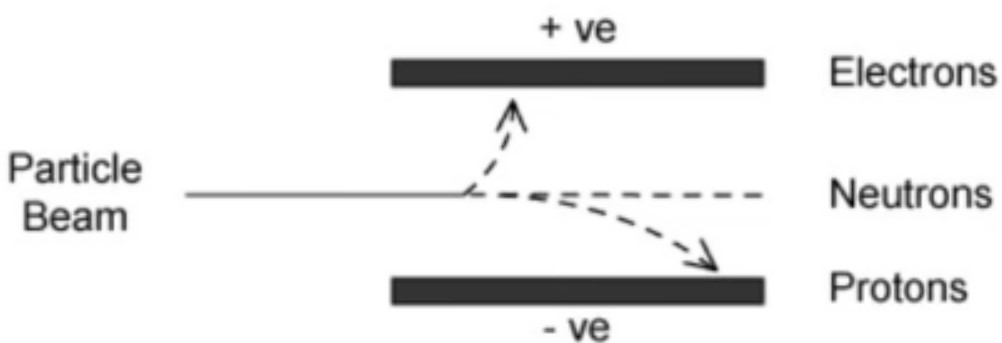
\includegraphics[width=10cm]{images/sub_particle_deflectn.jpg}
    \caption{Deflection of subatomic particles in electric field}
\end{figure}

\subsubsection{Isotopes}

\begin{defn}{Isotope}{}
Atom of same element with same number of protons but different number of neutrons.
\end{defn}

Isotopes have similar chemical properties since they have the same number of protons and hence the same number of electrons. 

However, their physical properties differ since they have different numbers of neutrons and hence different masses.

To distinguish among the isotopes present, a classification system has been devised. In this system, the nuclide of an element is represented as such:
\[ ^A_Z X \]
where $X$ denotes atomic symbol of the element in the periodic table, $Z$ denotes the atomic number/proton number (number of protons in the nucleus), $A$ denotes mass number/nucleon number (number of protons and neutrons in the nucleus).

\subsection{Electronic structure}

\begin{defn}{Orbital}{}
Region in space where there is high probability of finding an electron.
\end{defn}



\subsection{Electronic configuration}
\textbf{Ground state}: electron occupy orbitals of lowest available energy levels

\textbf{Excited state}: electron absorbs energy, promoted to higher energy level. Such atoms are unstable, release energy to return to ground state

Rules of orbital filling
\begin{enumerate}
\item \textbf{Aufbau principle}

Electrons occupy lowest energy orbitals first before higher energy orbitals -- filled in the order of increasing orbital energy.
(4s filled before, removed before 3d)

\item \textbf{Hund's rule}

Electrons added into orbitals singly first with parallel spins before pairing. 
(electrons positioned as far apart as possible to minimise inter-electronic repulsion)

\item \textbf{Pauli exclusion principle}

Each orbital holds max 2 electrons in opposite spins.
\end{enumerate}

Exceptions\footnote{You need to know these!}:
\begin{itemize}
\item \textbf{Chromium}: [Ar]$\unit{3d^5\,4s^1}$ instead of [Ar]$\unit{3d^4\,4s^2}$

to minimise inter-electronic repulsion

\item \textbf{Copper}: [Ar]$\unit{3d^{10}\,4s^1}$ instead of [Ar]$\unit{3d^9\,4s^2}$

fully filled 3d shells are stable due to symmetrical charge distribution
\end{itemize}


\subsection{Atomic trends}
\begin{defn}{First ionisation energy}{}
Energy required to remove 1 mole of electrons from 1 mole of gaseous atoms of the element to form 1 mole of singly charged gaseous cations.
\end{defn}

\begin{defn}{Second ionisation energy}{}
Energy required to remove 1 mole of electrons from 1 mole of singly positively charged gaseous ions to form 1 mole of doubly charged gaseous cations.
\end{defn}

\begin{defn}{Nuclear charge}{}
Electrostatic attraction of protons in nucleus on surrounding electrons.
\end{defn}

\begin{defn}{Shielding effect}{}
Partial decrease in electrostatic attraction of nucleus on valence electrons due to repulsive forces from other electrons.
\end{defn}

\begin{defn}{Effective nuclear charge}{}
Net electrostatic attraction of protons in nucleus on valence electrons.
\end{defn}
\pagebreak